\documentclass[tikz,border=10pt]{standalone}
\usepackage{amsmath,amssymb}
\usepackage{pgfplots}
\pgfplotsset{compat=1.18}
\usetikzlibrary{arrows.meta,positioning,calc,shapes}

\definecolor{politoNavy}{RGB}{0, 43, 91}
\definecolor{deepdiveTeal}{RGB}{0, 128, 128}
\definecolor{examred}{RGB}{180, 40, 40}
\definecolor{intuitiongreen}{RGB}{40, 130, 80}

\begin{document}
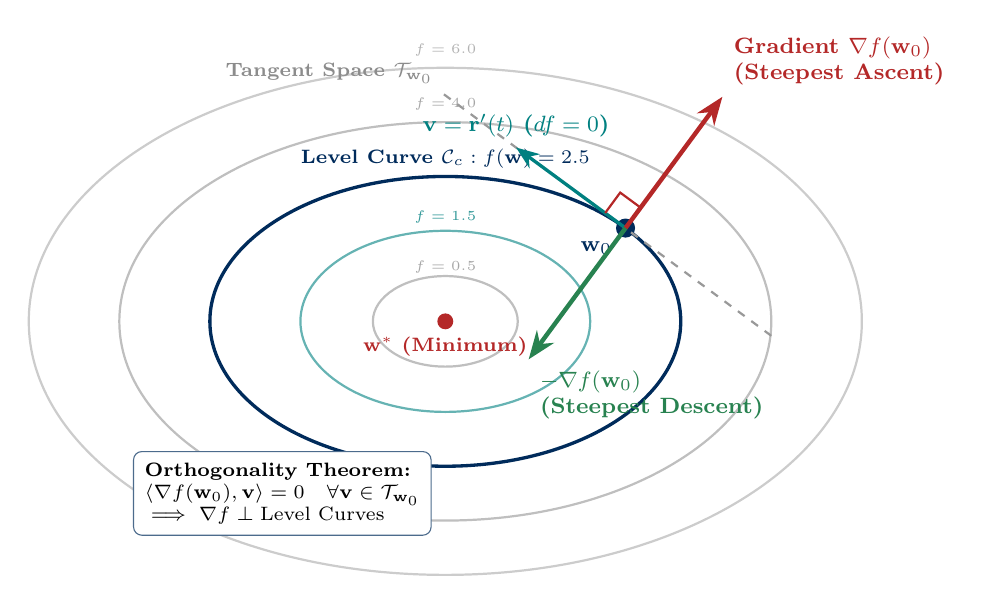
\begin{tikzpicture}[>=Stealth, scale=1.15]
  % Concentric elliptical contours of f(x,y)
  \draw[thick, gray!50] (0,0) ellipse (0.8cm and 0.5cm);
  \node[font=\tiny, gray!70] at (0, 0.6) {$f=0.5$};

  \draw[thick, deepdiveTeal!60] (0,0) ellipse (1.6cm and 1.0cm);
  \node[font=\tiny, deepdiveTeal!80] at (0, 1.15) {$f=1.5$};

  \draw[very thick, politoNavy] (0,0) ellipse (2.6cm and 1.6cm);
  \node[font=\scriptsize\bfseries, politoNavy] at (0, 1.8) {Level Curve $\mathcal{C}_c: f(\mathbf{w}) = 2.5$};

  \draw[thick, gray!50] (0,0) ellipse (3.6cm and 2.2cm);
  \node[font=\tiny, gray!70] at (0, 2.4) {$f=4.0$};

  \draw[thick, gray!40] (0,0) ellipse (4.6cm and 2.8cm);
  \node[font=\tiny, gray!60] at (0, 3.0) {$f=6.0$};

  % Center minimum
  \fill[examred] (0,0) circle (2.5pt);
  \node[below=2pt, font=\scriptsize\bfseries, text=examred] at (0,0) {$\mathbf{w}^*$ (Minimum)};

  % Marked point on level curve at angle 45 deg
  % Point on ellipse x = a*cos(t), y = b*sin(t)
  % For a=2.6, b=1.6, t=40 deg: x = 1.99, y = 1.03
  \coordinate (P) at (1.99, 1.03);
  \fill[politoNavy] (P) circle (3pt);
  \node[below left=2pt, font=\footnotesize\bfseries, text=politoNavy] at (P) {$\mathbf{w}_0$};

  % Tangent vector v: dx/dt = -a*sin(t), dy/dt = b*cos(t)
  % -2.6*sin(40) = -1.67, 1.6*cos(40) = 1.23
  % Normalized direction: (-1.67, 1.23) / 2.07 = (-0.805, 0.593)
  % Tangent line:
  \draw[thick, dashed, gray!80] ($(P) + (1.61, -1.19)$) -- ($(P) + (-2.01, 1.48)$)
    node[above left, font=\scriptsize\bfseries, text=gray!90] {Tangent Space $\mathcal{T}_{\mathbf{w}_0}$};

  % Tangent vector v arrow
  \draw[->, very thick, deepdiveTeal] (P) -- ($(P) + (-1.21, 0.89)$)
    node[above, font=\footnotesize\bfseries, text=deepdiveTeal] {$\mathbf{v} = \mathbf{r}'(t)$ ($df = 0$)};

  % Gradient vector: normal to tangent: (0.593, 0.805)
  % Uphill gradient arrow
  \draw[->, line width=1.6pt, examred] (P) -- ($(P) + (1.07, 1.45)$)
    node[above right, font=\footnotesize\bfseries, text=examred, align=left] {Gradient $\nabla f(\mathbf{w}_0)$\\(Steepest Ascent)};

  % Downhill negative gradient arrow
  \draw[->, line width=1.6pt, intuitiongreen] (P) -- ($(P) + (-1.07, -1.45)$)
    node[below right, font=\footnotesize\bfseries, text=intuitiongreen, align=left] {$-\nabla f(\mathbf{w}_0)$\\(Steepest Descent)};

  % Right angle symbol between v and grad f
  % unit tangent: u_t = (-0.805, 0.593)
  % unit normal: u_n = (0.593, 0.805)
  \coordinate (RA1) at ($(P) + 0.28*(-0.805, 0.593)$);
  \coordinate (RA2) at ($(P) + 0.28*(-0.805, 0.593) + 0.28*(0.593, 0.805)$);
  \coordinate (RA3) at ($(P) + 0.28*(0.593, 0.805)$);
  \draw[thick, examred] (RA1) -- (RA2) -- (RA3);

  % Mathematical theorem annotation
  \node[draw=politoNavy!70, fill=white, rounded corners=3pt, inner sep=4pt, font=\scriptsize, align=left] at (-1.8, -1.9) {
    \textbf{Orthogonality Theorem:}\\
    $\langle \nabla f(\mathbf{w}_0), \mathbf{v} \rangle = 0 \quad \forall \mathbf{v} \in \mathcal{T}_{\mathbf{w}_0}$\\
    $\implies \nabla f \perp \text{Level Curves}$
  };
\end{tikzpicture}
\end{document}
